\documentclass[12pt,aspectratio=169]{beamer}

\usetheme{metropolis}

\definecolor{mDarkBrown}{HTML}{FF5722}
\definecolor{mDarkTeal}{HTML}{263238}
\definecolor{mLightBrown}{HTML}{FF5722}

\usepackage{booktabs}
\usepackage{graphicx}
\usepackage{hyphenat}
\usepackage{multirow}
\usepackage{nicefrac}
\usepackage[normalem]{ulem}

\usepackage[weather]{ifsym}

\usepackage{pifont}
\newcommand{\cmark}{\ding{51}}
\newcommand{\xmark}{\ding{55}}

\usepackage{minted}
\usemintedstyle{tango}
\newminted[bash]{bash}{%
    autogobble,
    bgcolor=mDarkTeal!10,
    linenos
}
\newminted[py3]{python}{%
    python3,
    autogobble,
    bgcolor=mDarkTeal!10,
    linenos
}
\newminted[sql]{sql}{%
    autogobble,
    bgcolor=mDarkTeal!10,
    linenos
}

\usepackage{polyglossia}
\setdefaultlanguage[variant=british]{english}
\usepackage[english=british]{csquotes}

\defaultfontfeatures{Ligatures=TeX}
\setmainfont{Lucida Sans OT}
\setsansfont[Scale=MatchLowercase]{Lucida Sans OT}
\setmonofont[Scale=MatchLowercase]{Lucida Console DK}

\usepackage{mathspec}
\setmathsfont(Digits,Latin,Greek)[Numbers={Lining,Proportional}]{Lucida Bright Math OT}

\newcommand{\mat}[1]{\ensuremath{\mathbf{#1}}}

\newcommand{\R}{\ensuremath{\mathbb{R}}}

\newcommand{\E}[1]{\ensuremath{\mathbb{E}\!\left[ #1 \right]}}
\newcommand{\V}[1]{\ensuremath{\mathbb{V}\!\left[ #1 \right]}}
\newcommand{\Prob}[1]{\ensuremath{\Pr\!\left( #1 \right)}}
\newcommand{\Normal}[2]{\ensuremath{\mathcal{N}\!\left( #1, #2 \right)}}
\newcommand{\simiid}{\ensuremath{\overset{\text{\tiny i.i.d.}}{\sim}}}

\DeclareMathOperator{\logit}{logit}

\author{Gianluca Campanella}
\date{}



\title{Probability theory and statistics}

\begin{document}

\maketitle

\begin{frame}{Contents}
    \tableofcontents[hideallsubsections]
\end{frame}

\section{Probability theory}

\begin{frame}{`Random' points}
    \begin{center}
        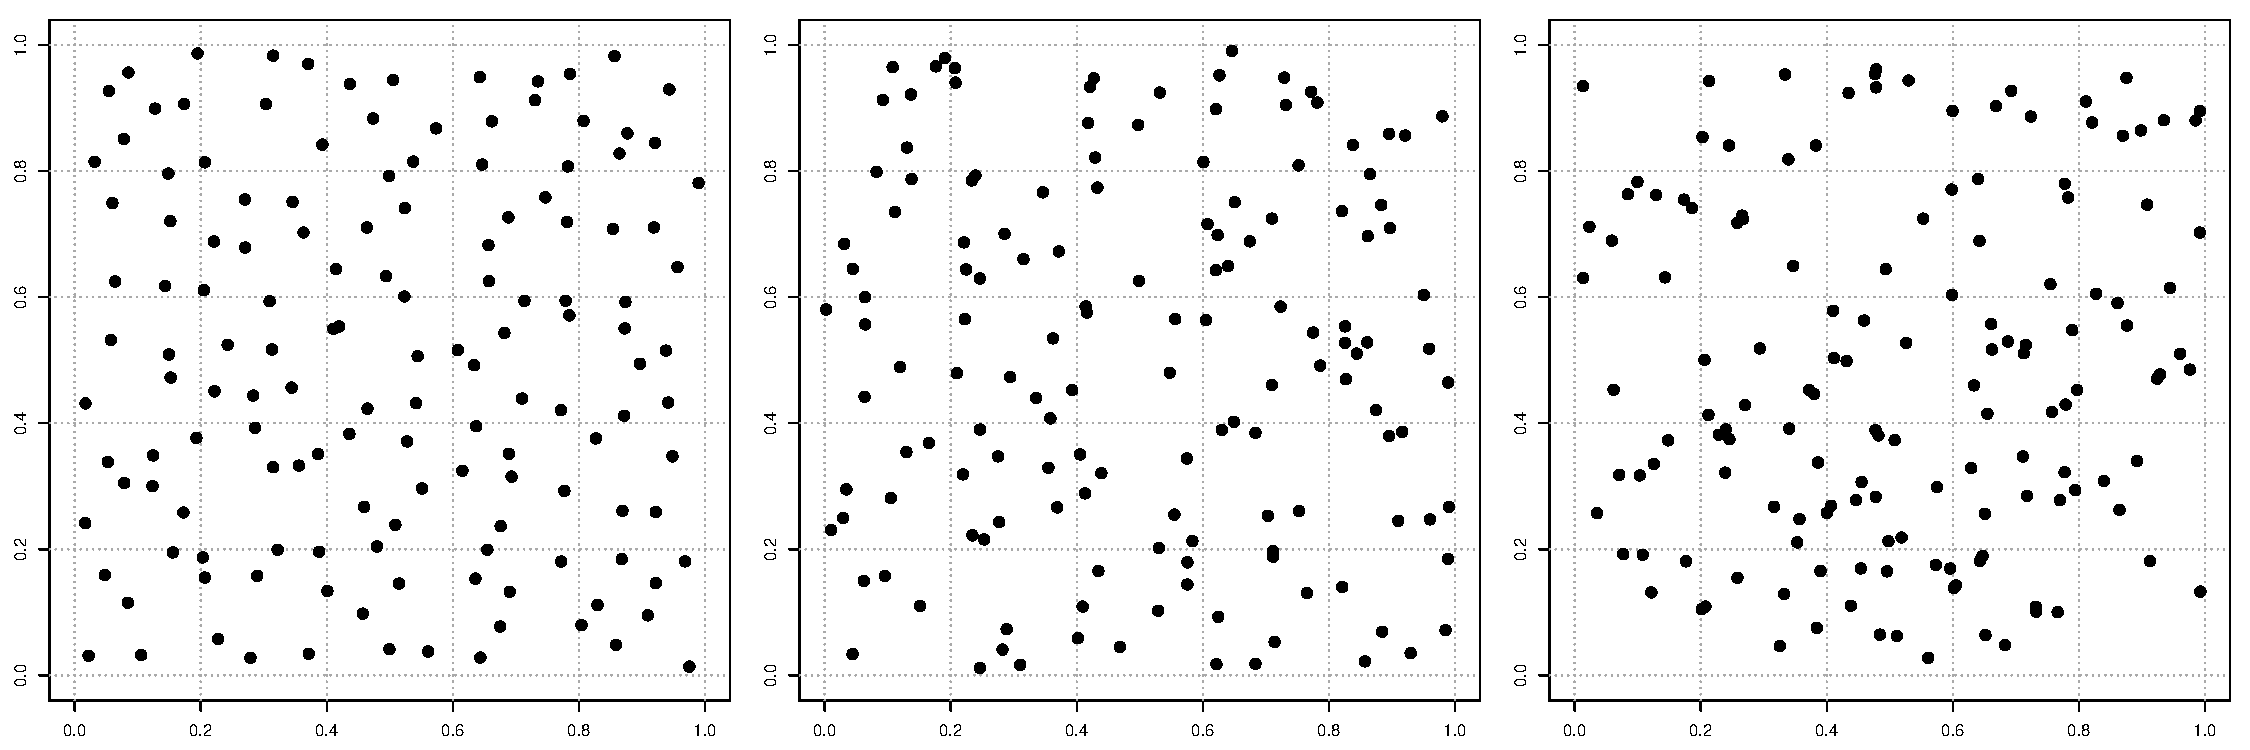
\includegraphics[width=\textwidth]{figures/random_points}
    \end{center}
\end{frame}

\begin{frame}{What is probability?}
    \begin{quote}
        `The extent to which something is likely to happen'
        \begin{flushright}
            \small%
            --- Oxford English Dictionary
        \end{flushright}
    \end{quote}
    \vfill
    \begin{block}{Examples}
        \begin{itemize}
            \item Probability that it will rain tomorrow
            \item Probability that you will win the lottery
        \end{itemize}
    \end{block}
\end{frame}

\begin{frame}{Sources of uncertainty}
    \begin{columns}[t]
        \begin{column}{0.5\textwidth}
            \begin{center}
                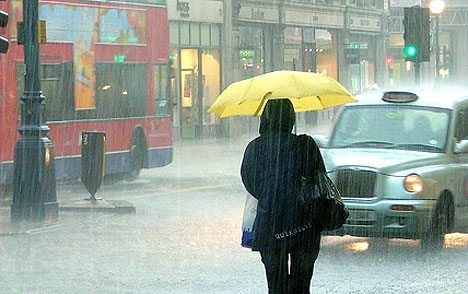
\includegraphics[height=2cm]{figures/rain} \\[\medskipamount]
                \alert{Imperfect information}
            \end{center}
            Current predictive tools can only assign a number indicating our
            degree of certainty
        \end{column}
        \begin{column}{0.5\textwidth}
            \begin{center}
                
\includegraphics[height=2cm]{figures/lottery} \\[\medskipamount]
                \alert{Stochastic process}
            \end{center}
            The experiment is designed to produce uncertain results (because
            it's fun)
        \end{column}
    \end{columns}
\end{frame}

\begin{frame}{Probability theory}
    \begin{block}{What?}
        The branch of mathematics concerned with \alert{random phenomena}
    \end{block}
    \vfill\pause
    \begin{block}{How?}
        Using mathematical \alert{abstractions} of non\hyp{}deterministic events
    \end{block}
    \vfill\pause
    \begin{block}{Why?}
        To identify \alert{patterns} in (apparently) random occurrences
    \end{block}
\end{frame}

\begin{frame}{Statistical regularity}
    \only<1>{%
        \begin{center}
            {\LARGE%
             We cannot predict with certainty \\ if it's going to rain tomorrow}
            \vfill
            {\large%
             but}
            \vfill
            {\LARGE%
             we can predict `average behaviour'}
        \end{center}}
    \only<2>{%
        In summary\ldots
        \begin{itemize}
            \item Probability theory describes the behaviour of random phenomena
                  \alert{in the long run}
            \item If this information is useful, probability theory can be a
                  valuable tool for \alert{decision-making}
        \end{itemize}}
\end{frame}

\begin{frame}[t]{Random variables `encapsulate' random events}
    \begin{block}{Notation}
        \begin{itemize}
            \item $X$, $Y$, \ldots~(upper case) are \alert{random variables}
            \item $X = x$ (lower case) is a value (\alert{realisation}) of $X$
            \item $\Prob{X = x}$ is the \alert{probability} that $X = x$
        \end{itemize}
    \end{block}
    \vfill
    \begin{block}{Example}
        \begin{itemize}
            \item $X$ represents the (`archetypal') outcome of a coin toss
            \item $X = \text{`head'}$ represents one (actual) outcome
            \item $\Prob{X = \text{`head'}}$ is the long\hyp{}term probability
                  of the outcome `head'
        \end{itemize}
    \end{block}
\end{frame}

\begin{frame}{Maximum of two fair dice}
    \begin{columns}[t]
        \begin{column}{0.5\textwidth}
            \centering
            \textbf{A fair die} \\[\bigskipamount]
            \begin{tabular}{cc}
                \toprule
                $x$ & $\Prob{X = x}$ \\
                \midrule
                $1$ & $1/6$ \\
                $2$ & $1/6$ \\
                $3$ & $1/6$ \\
                $4$ & $1/6$ \\
                $5$ & $1/6$ \\
                $6$ & $1/6$ \\
                \bottomrule
            \end{tabular}
        \end{column}
        \begin{column}{0.5\textwidth}
            \centering
            \textbf{Maximum of two fair dice} \\[\bigskipamount]
            \begin{itemize}
                \item How many outcomes?
                \item $\Prob{X = 1}$?
                \item $\Prob{X = 6}$?
            \end{itemize}
        \end{column}
    \end{columns}
\end{frame}

\begin{frame}{Probability distributions}
    \begin{center}
        \large%
        \textbf{Simplified approximations to reality}
    \end{center}
    \vfill
    \begin{itemize}
        \item Detailed enough to capture important characteristics and serve as
              \alert{prediction tools}
        \item Simple enough to be usable in practice
    \end{itemize}
\end{frame}

\begin{frame}{Characterising probability distributions}
    \begin{block}{Measures of central tendency}
        \begin{itemize}
            \item (Arithmetic) mean or average
            \item Median
            \item Mode
        \end{itemize}
    \end{block}
    \vfill\pause
    \begin{block}{Measures of dispersion}
        \begin{itemize}
            \item Variance
            \item Minimum and maximum $\rightarrow$ range
            \item Quantiles (a.k.a.\ order statistics)
        \end{itemize}
    \end{block}
\end{frame}

\begin{frame}{Characterising probability distributions}
    \begin{center}
        \large%
        1, 8, 16, 30, 32, 37, 53, 80, 86, 91, 93
    \end{center}
    \vfill
    \begin{itemize}
        \item Mean?
        \item Median?
        \item Mode?
        \item Variance and standard deviation?
        \item Minimum and maximum, and range?
        \item Quartiles?
    \end{itemize}
\end{frame}

\section{Statistics}

\begin{frame}{Statistics}
    \begin{block}{What?}
        The science of collecting and analysing numerical data
    \end{block}
    \vfill\pause
    \begin{block}{How?}
        By planning studies, exploring and modelling the data using the tools of
        \alert{probability theory}
    \end{block}
    \vfill\pause
    \begin{block}{Why?}
        To infer properties of a \alert{population} from a \alert{sample}
    \end{block}
\end{frame}

\begin{frame}[t]{Probability or statistics?}
    You have a fair coin. You toss it 100 times. \\
    How likely is it to land heads 60 times or more?
    \vfill\pause
    \begin{center}
        \large%
        \textbf{Probability}
    \end{center}
    \begin{itemize}
        \item Random process is known (or assumed): `fair coin'
        \item Objective: \alert{find probability of a certain outcome}
    \end{itemize}
\end{frame}

\begin{frame}[t]{Probability or statistics?}
    I give you a coin. You toss it 100 times and count 60 heads. \\
    Is the coin fair?
    \vfill\pause
    \begin{center}
        \large%
        \textbf{Statistics}
    \end{center}
    \begin{itemize}
        \item Outcome is known (or measured): `$60 / 100$ heads'
        \item Objective: \alert{characterise the random process}
    \end{itemize}
\end{frame}

\begin{frame}{Probability theory and statistics}
    \begin{columns}[t]
        \begin{column}{0.5\textwidth}
            \begin{center}
                \textbf{Probability theory}
            \end{center}
            \begin{itemize}
                \item Defines the model
                \item \ldots and often its \alert{parameters}
            \end{itemize}
        \end{column}
        \begin{column}{0.5\textwidth}
            \begin{center}
                \textbf{Statistics}
            \end{center}
            \begin{itemize}
                \item Collects the data
                \item `Fits' the model \\ (estimates its parameters)
                \item Makes \alert{inferences}
            \end{itemize}
        \end{column}
    \end{columns}
\end{frame}

\end{document}

